\subsubsection{Réseau de neurones récurrent (RNN)}
Jusque maintenant, nous avons vu des réseaux de neurones \emph{feedforward}.
C'est à dire qu'ils ne présentent aucune boucle. Mais il éxiste des réseaux de neurones présentant des boucles.
Cela leur permet de prendre en compte les entrées précédentes.
\ssstitle{Structure}
\begin{figure}
 \centering
 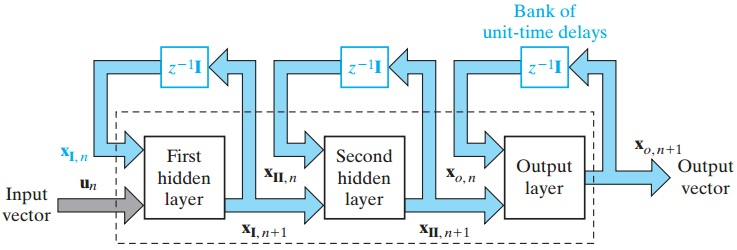
\includegraphics[scale=0.5]{../figures/structurermlp.jpg}
 \caption{Structure RLMP. \textbf{Source}: Haykin. p795\cite{Haykin}}
 \label{structurermlp}
\end{figure}
\begin{figure}
 \centering
 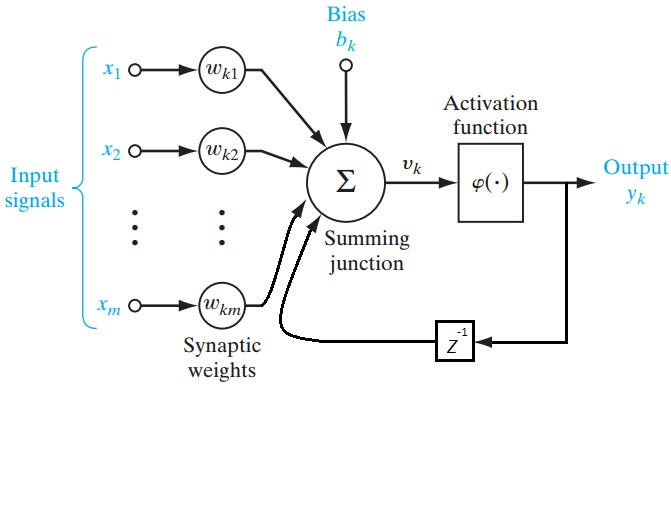
\includegraphics[scale=0.5]{../figures/neuronermlp.jpg}
 \caption{Neurone caché d'un RMLP}
 \label{neuronermlp}
\end{figure}
Un réseau de neurones récurrent est un réseaux présentant des boucles dans sa structure.
Des \emph{délais} notés $Z^{-1}$ sont présents sur certains arcs dans le réseau afin de retarder d'une étape, la transmission d'une valeur.
Une étape dans un réseau consiste à recevoir une entrée et de générer une sortie.
Il existe plusieurs réseaux de type récurrent (récurrent simple, machine à états liquide, etc).
La Figure \ref{structurermlp} présente un réseau de type perceptron multi-couches récurrent (\rmlp).
Il s'agit d'un \mlp dont les neurones des couches cachées ont un arc qui boucle sur le neurone lui-même avec un $Z^{-1}$ sur cet arc, comme sur la Figure \ref{neuronermlp}.
\ssstitle{Applications}
Grâce aux délais, le réseau peut approximer des fonctions dont la sortie ne dépend pas seulement de l'entrée actuelle mais aussi des entrées précédentes.
Mais cette fonctionnalité n'est pas utile pour notre application puisque les commandes à générer ne dépendent pas des états précédents l'état actuel.
%Les \emph{machines à états liquides} (\lsm), dont les connections se font de manière aléàtoire, sont utilisés pour la reconnaissance automatique de la parole. %TODO citer
%Les \emph{long-short term memory} sont utilisés pour la reconnaissance automatique de la parole ou de l'écriture manuscrite. %TODO citer